%% ===================================================================
\section{Results}
\label{sec:results}

\subsection{Corpus and ray-budget convergence}
\label{sec:res-corpus}

The corpus contains \nCities{} cities, \nBuildings{} buildings,
\nSites{} sites and \nSamples{} ray-traced links (Table~\ref{tab:corpus});
\nTiles{} tiles have at least \minLinks{} links and are labelled.
Figure~\ref{fig:city} shows one city. The share of buildings whose height
is imputed from the city median ranges from \impMin\% (\impMinCity) to
\impMax\% (\impMaxCity).

The radio-map solver is a Monte-Carlo method: a cell that no ray reaches
reports zero power, so the set of reached cells and their values depend on
the ray budget. Table~\ref{tab:convergence} compares budgets with a
reference run of \convRef{} rays for one site. At the \rtSamples{} rays per
site used for the corpus, path loss below \SI{120}{\decibel} agrees with the
reference to \SI{\convRmsOneTwenty}{\decibel} RMS and path loss below
\SI{140}{\decibel} to \SI{\convRmsOneForty}{\decibel} with a mean difference
of \SI{\convBiasOneForty}{\decibel}, and the number of cells reached below \SI{140}{\decibel} is
\convCellsOneForty\% of the reference. The complete corpus
took \rtHours{}\,h on a \rtBackend{} backend (\rtSecPerSite{}\,s per site).

\begin{table*}[!t]
\centering
\caption{Corpus. Height source: share of buildings with an explicit height
attribute, with a floor count, or imputed from the city median. Links: ray-traced
(pixel, site) pairs below the \SI{\maxPl}{\decibel} cut-off. Tiles: labelled
tiles ($\ge\minLinks{}$ links).}
\label{tab:corpus}
\small
% generated by paper/scripts/make_assets.py
\begin{tabular}{lrrrrrrr}
\toprule
& & \multicolumn{3}{c}{Height source (\%)} & & & \\
\cmidrule(lr){3-5}
City & Buildings & tag & storeys & imputed & Median (m) & Links & Tiles \\
\midrule
Amsterdam & 21{,}135 & 83 & 2 & 15 & 15.5 & 736{,}255 & 948 \\
Barcelona & 12{,}337 & 12 & 64 & 23 & 19.2 & 609{,}050 & 942 \\
Berlin & 6{,}036 & 15 & 63 & 22 & 16.0 & 1{,}009{,}619 & 957 \\
Chicago & 2{,}952 & 70 & 4 & 25 & 15.9 & 1{,}069{,}552 & 961 \\
Hamburg & 4{,}335 & 17 & 42 & 41 & 16.0 & 1{,}152{,}125 & 961 \\
London & 11{,}891 & 8 & 42 & 50 & 12.8 & 931{,}288 & 940 \\
Munich & 8{,}616 & 9 & 49 & 42 & 12.8 & 794{,}056 & 950 \\
New York & 7{,}126 & 98 & 1 & 2 & 18.6 & 827{,}510 & 960 \\
Paris & 14{,}383 & 3 & 64 & 33 & 19.2 & 529{,}649 & 910 \\
Prague & 9{,}907 & 1 & 70 & 29 & 16.0 & 783{,}805 & 960 \\
Vienna & 7{,}082 & 26 & 60 & 14 & 16.0 & 534{,}491 & 939 \\
\midrule
Total & 105{,}800 & & & & & 8{,}977{,}400 & 10{,}428 \\
\bottomrule
\end{tabular}

\end{table*}

\begin{table*}[!t]
\centering
\caption{Ray-budget convergence for one site (\figCity{}, \SI{\cellSize}{\metre}
cells). For each path-loss level: number of cells reached below that level,
relative to the \convRef{}-ray reference (\%; Monte-Carlo noise can exceed
100\%), and RMS path-loss difference to the reference over the cells reached
by both (dB). s: solver time.}
\label{tab:convergence}
\small
% generated by paper/scripts/make_assets.py
\begin{tabular}{rrrrrrrrrr}
\toprule
& & \multicolumn{2}{c}{$\le120$\,dB} & \multicolumn{2}{c}{$\le130$\,dB} & \multicolumn{2}{c}{$\le140$\,dB} & \multicolumn{2}{c}{$\le150$\,dB} \\
\cmidrule(lr){3-4}\cmidrule(lr){5-6}\cmidrule(lr){7-8}\cmidrule(lr){9-10}
Rays & s & cells & RMS & cells & RMS & cells & RMS & cells & RMS \\
\midrule
\num{1e7} & 9 & 95.9 & 1.69 & 82.4 & 2.92 & 75.1 & 4.48 & 74.7 & 6.68 \\
\num{3e7} & 27 & 99.8 & 0.98 & 92.7 & 1.88 & 87.7 & 3.11 & 86.1 & 4.54 \\
\num{1e8} & 98 & 100.3 & 0.53 & 98.4 & 1.14 & 96.1 & 2.00 & 94.9 & 3.13 \\
\num{3e8} & 245 & 100.0 & 0.00 & 100.0 & 0.00 & 100.0 & 0.00 & 100.0 & 0.00 \\
\bottomrule
\end{tabular}

\end{table*}

\begin{figure*}[!t]
\centering
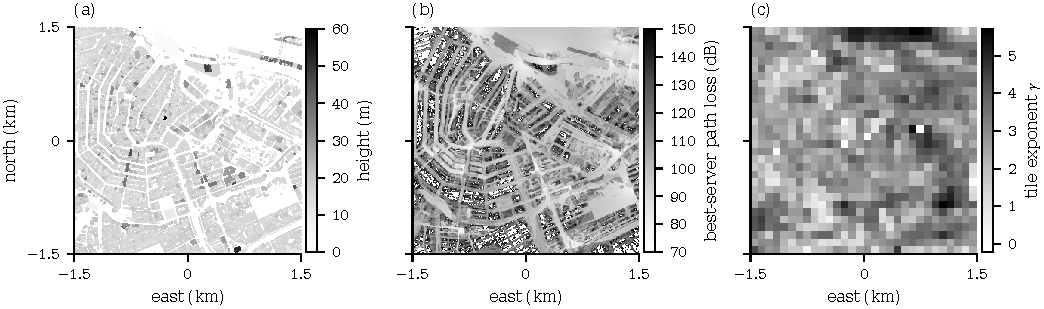
\includegraphics[width=\textwidth]{figures/fig_city.pdf}
\caption{\figCity{}. (a)~Building heights of the scene. (b)~Ray-traced path loss
to the best site. (c)~Tile exponents $\hat\gamma_t$.}
\label{fig:city}
\end{figure*}

\subsection{Tile labels and their precision}
\label{sec:res-labels}

Table~\ref{tab:fits} summarises the labels. City medians of the tile
exponent range from \gammaMedMin{} (\gammaMedMinCity) to \gammaMedMax{}
(\gammaMedMaxCity); their standard deviation across cities, \betweenSd, is
only \betweenWithinRatio{} times the typical standard deviation of the
tiles within a city (\withinSdMin--\withinSdMax). Most of the variation of
the tile exponent is therefore within cities, not between them. The fit
residual of the log-distance law inside a tile is
\fitRmseMin--\SI{\fitRmseMax}{\decibel}.

Without shrinkage, the OLS exponents span \olsMin{} to \olsMax{}, the
ill-conditioning predicted by Proposition~\ref{prop:identify}; empirical-Bayes
shrinkage (median weight \shrinkMedian) narrows this to \ebMin--\ebMax{}.
Label precision is the decisive quantity (Table~\ref{tab:noise}). The
standard error assuming independent residuals is \seIid; the
cluster-robust error with sites as clusters is \seCluster, \seRatio{} times
larger, and the split-half estimate extrapolated to the full data is
\seSplit. The exponent of a tile therefore depends strongly on which sites
serve it, and a label error of this size is comparable to the differences
between cities.

\begin{table*}[!t]
\centering
\caption{Tile labels per city. City-wide fit: OLS over all links. Tile labels:
median and standard deviation of $\hat\gamma_t$ and median $\hat P_{L_0,t}$
(dB, at $d_0=\SI{\refDist}{\metre}$); $\hat\tau$: between-tile standard deviation
of the slope; $w_t$: shrinkage weight; RMSE: link-weighted fit residual (dB).}
\label{tab:fits}
\small
% generated by paper/scripts/make_assets.py
\begin{tabular}{lrrrrrrrr}
\toprule
& \multicolumn{2}{c}{City-wide fit} & \multicolumn{3}{c}{Tile labels} & & & \\
\cmidrule(lr){2-3}\cmidrule(lr){4-6}
City & $\gamma$ & $P_{L_0}$ & med.\ $\gamma$ & s.d.\ $\gamma$ & med.\ $P_{L_0}$ & $\hat\tau$ & med.\ $w_t$ & RMSE \\
\midrule
Amsterdam & 2.47 & 100.5 & 2.84 & 0.93 & 100.9 & 1.06 & 0.27 & 11.3 \\
Barcelona & 1.92 & 105.4 & 2.43 & 0.96 & 105.5 & 1.14 & 0.28 & 11.6 \\
Berlin & 2.65 & 98.2 & 2.82 & 0.81 & 97.5 & 1.00 & 0.36 & 11.6 \\
Chicago & 0.81 & 115.6 & 2.79 & 0.83 & 97.2 & 1.19 & 0.54 & 12.7 \\
Hamburg & 2.14 & 100.2 & 3.15 & 0.72 & 92.2 & 0.94 & 0.37 & 11.4 \\
London & 1.72 & 104.4 & 2.40 & 0.60 & 103.3 & 0.79 & 0.42 & 11.2 \\
Munich & 2.12 & 104.0 & 3.00 & 0.80 & 99.8 & 0.92 & 0.33 & 11.2 \\
New York & 1.11 & 115.9 & 2.69 & 0.79 & 102.2 & 1.18 & 0.53 & 12.6 \\
Paris & 2.06 & 103.6 & 2.41 & 0.95 & 106.7 & 1.13 & 0.29 & 11.8 \\
Prague & 2.48 & 100.9 & 2.92 & 0.77 & 99.0 & 0.95 & 0.37 & 11.4 \\
Vienna & 2.29 & 106.1 & 2.39 & 0.92 & 108.4 & 1.09 & 0.32 & 11.4 \\
\bottomrule
\end{tabular}

\end{table*}

\begin{table}[!t]
\centering
\caption{Standard error of the tile labels: independent residuals (iid),
cluster-robust over sites (cluster), and split-half over random halves of the
sites extrapolated to all sites (split). Root mean square over tiles.}
\label{tab:noise}
\scriptsize\setlength{\tabcolsep}{2.4pt}
% generated by paper/scripts/make_assets.py
\begin{tabular}{lrrrrrrr}
\toprule
& & \multicolumn{3}{c}{$\mathrm{se}(\gamma)$} & \multicolumn{3}{c}{$\mathrm{se}(P_{L_0})$ (dB)} \\
\cmidrule(lr){3-5}\cmidrule(lr){6-8}
City & sites/tile & iid & cluster & split & iid & cluster & split \\
\midrule
Amsterdam & 18 & 0.140 & 0.440 & 0.600 & 1.42 & 5.06 & 6.90 \\
Barcelona & 18 & 0.178 & 0.470 & 0.592 & 1.73 & 5.31 & 6.91 \\
Berlin & 19 & 0.131 & 0.445 & 0.583 & 1.50 & 5.34 & 6.99 \\
Chicago & 19 & 0.117 & 0.545 & 1.006 & 1.33 & 6.73 & 12.38 \\
Hamburg & 20 & 0.098 & 0.402 & 0.629 & 1.09 & 4.77 & 7.45 \\
London & 19 & 0.105 & 0.353 & 0.537 & 1.18 & 4.39 & 6.62 \\
Munich & 18 & 0.131 & 0.397 & 0.559 & 1.41 & 4.76 & 6.75 \\
New York & 17 & 0.142 & 0.541 & 0.890 & 1.54 & 6.65 & 10.40 \\
Paris & 17 & 0.187 & 0.488 & 0.651 & 1.91 & 5.57 & 7.56 \\
Prague & 19 & 0.115 & 0.416 & 0.667 & 1.25 & 4.84 & 7.45 \\
Vienna & 16 & 0.179 & 0.481 & 0.674 & 1.80 & 5.42 & 7.69 \\
\midrule
RMS & & 0.141 & 0.456 & 0.686 & 1.49 & 5.40 & 8.10 \\
\bottomrule
\end{tabular}

\end{table}

\begin{figure*}[!t]
\centering
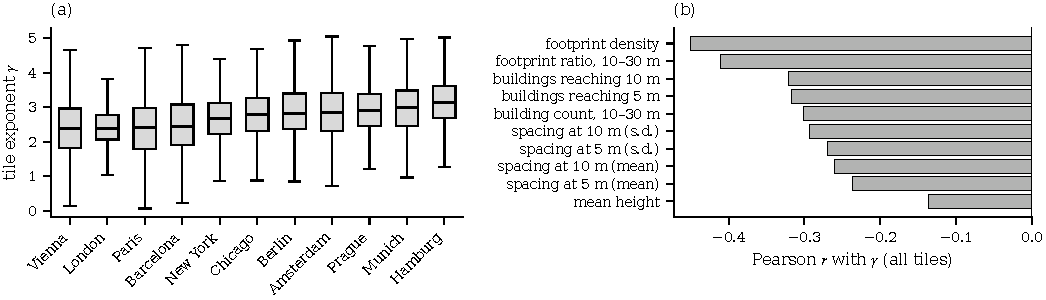
\includegraphics[width=\textwidth]{figures/fig_corpus.pdf}
\caption{(a)~Tile exponents per city (box: quartiles; whiskers: 1.5 times the
interquartile range). (b)~The ten descriptors most correlated with the tile
exponent over all \nTiles{} tiles.}
\label{fig:corpus}
\end{figure*}

The descriptors carry signal (Fig.~\ref{fig:corpus}b): the strongest single
correlation with the exponent is $r=\topDescR$ for \topDesc, and no
descriptor exceeds $|r|=\maxAbsR$.

\subsection{Zero-shot transfer of tile parameters}
\label{sec:res-loco}

Table~\ref{tab:loco} and Fig.~\ref{fig:loco} report the exponent error on
every held-out city. The source median attains \rmseMedian; kernel transfer
\rmseKernel; the Gaussian process with learned length scales \rmseGpArd; the
learned regressors \rmseRidge{} (ridge), \rmseMlp{} (MLP), \rmseEncoder{}
(neural encoder) and \rmseGbdt{} (GBDT). The domain-adaptation variants do
not improve on their base learners (CORAL \rmseCoral{} against ridge
\rmseRidge; GBDT-IW \rmseGbdtIw{} against GBDT \rmseGbdt), and the standard
models are worse than the median (3GPP UMa \rmseUmaLos{} and \rmseUmaNlos,
COST-231 Hata \rmseCost). The best operator is the \bestZeroShot. For the
intercept at \SI{\refDist}{\metre} the learned operators reduce the error
from \SI{\plRmseMedian}{\decibel} (median) to \SI{\plRmseGbdt}{\decibel}
(GBDT).

At the level of cities (Table~\ref{tab:stats-param}), GBDT improves on the median
by \dGbdtMedian{} (95\% CI [\loGbdtMedian, \hiGbdtMedian], $p=\pGbdtMedian$,
better in \nGbdtMedian{} of \nFolds{} cities) and on kernel transfer by
\dGbdtKernel{} ([\loGbdtKernel, \hiGbdtKernel]); kernel transfer does not
improve significantly on the median (\dKernelMedian, [\loKernelMedian,
\hiKernelMedian], $p=\pKernelMedian$), whereas learning the metric of the
same kernel does: GP-ARD improves on kernel transfer by \dGpKernel{}
([\loGpKernel, \hiGpKernel], better in \nGpKernel{} of \nFolds{} cities).
With eleven cities, none of these improvements is significant after Holm's
correction over the \nZeroShotTotal{} comparisons with the median; the only
significant differences are deteriorations (\zeroShotSigWorseList). The hardest target is \hardCity, where
the best operator reaches \hardCityBest.

\begin{table*}[!t]
\centering
\caption{Zero-shot exponent RMSE per held-out city (mean of five seeds for
stochastic operators; best per row in bold). Last row: mean $P_{L_0}$ RMSE (dB).}
\label{tab:loco}
\small
% generated by paper/scripts/make_assets.py
\begin{tabular}{lrrrrrrrrrrrrr}
\toprule
Target city & Median & UMa-L & UMa-N & COST & Kernel & GP & $k$-NN & Ridge & CORAL & MLP & Enc. & GBDT & IW \\
\midrule
Amsterdam & 0.949 & 1.146 & 1.394 & 1.035 & 0.843 & 0.784 & \textbf{0.761} & 0.786 & 0.820 & 0.781 & 0.788 & 0.793 & 0.801 \\
Barcelona & 1.002 & 0.998 & 1.730 & 1.318 & 0.900 & 0.777 & 0.811 & 0.795 & 0.817 & \textbf{0.777} & 0.781 & 0.882 & 0.895 \\
Berlin & 0.834 & 1.052 & 1.319 & 0.946 & 0.783 & 0.751 & 0.775 & 0.761 & 0.877 & 0.758 & \textbf{0.750} & 0.756 & 0.756 \\
Chicago & \textbf{0.835} & 1.006 & 1.414 & 1.031 & 0.938 & 0.894 & 0.960 & 0.908 & 0.876 & 0.900 & 0.893 & 0.878 & 0.871 \\
Hamburg & 0.850 & 1.162 & 1.078 & 0.770 & 0.717 & 0.631 & 0.630 & 0.629 & 0.616 & \textbf{0.614} & 0.629 & 0.739 & 0.668 \\
London & 0.683 & 0.639 & 1.599 & 1.097 & 0.631 & 0.637 & 0.697 & 0.626 & \textbf{0.624} & 0.634 & 0.648 & 0.661 & 0.669 \\
Munich & 0.860 & 1.120 & 1.229 & 0.875 & 0.775 & 0.777 & 0.784 & 0.771 & 0.806 & 0.764 & \textbf{0.764} & 0.766 & 0.766 \\
New York & \textbf{0.792} & 0.907 & 1.489 & 1.064 & 0.966 & 0.842 & 0.847 & 0.870 & 0.860 & 0.851 & 0.844 & 0.828 & 0.877 \\
Paris & 1.005 & 0.977 & 1.748 & 1.308 & 0.845 & 0.816 & 0.836 & 0.809 & 0.818 & 0.808 & 0.809 & \textbf{0.806} & 0.811 \\
Prague & 0.807 & 1.086 & 1.219 & 0.851 & 0.691 & 0.672 & 0.675 & 0.673 & 0.733 & \textbf{0.669} & 0.683 & 0.673 & 0.683 \\
Vienna & 0.968 & 0.938 & 1.761 & 1.302 & 0.853 & 0.826 & 0.839 & 0.828 & \textbf{0.805} & 0.820 & 0.847 & 0.826 & 0.824 \\
\midrule
Mean & 0.871 & 1.003 & 1.453 & 1.054 & 0.813 & 0.764 & 0.783 & 0.769 & 0.787 & \textbf{0.761} & 0.767 & 0.782 & 0.784 \\
S.d. & 0.100 & 0.147 & 0.234 & 0.191 & 0.105 & 0.085 & 0.092 & 0.092 & 0.091 & 0.089 & 0.084 & 0.073 & 0.083 \\
\midrule
$P_{L_0}$ (dB) & 13.8 & 21.6 & 13.8 & 17.9 & 10.5 & 9.5 & 9.8 & 9.7 & 10.3 & 9.5 & 9.6 & 9.6 & 9.6 \\
\bottomrule
\end{tabular}

\end{table*}

\begin{figure}[!t]
\centering
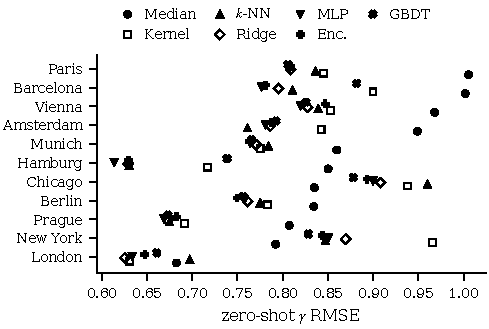
\includegraphics[width=\linewidth]{figures/fig_loco.pdf}
\caption{Zero-shot exponent RMSE per held-out city, ordered by the error of the
source median.}
\label{fig:loco}
\end{figure}

\subsection{Regime of kernel transfer}
\label{sec:res-kernel}

Table~\ref{tab:degeneracy} places the tuned kernel operator relative to
Theorem~\ref{thm:regimes}. The selected bandwidths are
$\sigma=\sigmaMin$--$\sigmaMax$ and the median $\epsilon_u$ ranges from
\epsMedianMin{} to \epsMedianMax: no target tile satisfies the condition of
part~(a), and the largest single weight has median \wmaxMedian, so the
operator is not a nearest-neighbour copy either. Where the largest bandwidth
is selected, however, it averages over up to \neffFracMax\% of the source
tiles and its predictions spread over as little as \spreadMin{} of the spread of
the target labels: it approaches the source mean although part~(a) does not
hold. Across the targets the prediction spread is
\spreadMin--\spreadMax{} of that of the labels. Its disadvantage is the
noise-transmission term of Proposition~\ref{prop:decomp} combined with an
isotropic distance in which every descriptor counts equally; the Gaussian
process, which learns one length scale per descriptor, removes most of the
gap to the learned regressors (Section~\ref{sec:res-loco}).

\begin{table}[!t]
\centering
\caption{Kernel transfer on each held-out city: selected bandwidth; median
$\epsilon_u=D_u/2\sigma^2$ and share of tiles with $\epsilon_u<1$
(Theorem~\ref{thm:regimes}a); median effective-neighbourhood fraction; median
largest weight (Theorem~\ref{thm:regimes}b); standard deviation of the
predictions over that of the labels.}
\label{tab:degeneracy}
\small\setlength{\tabcolsep}{2.5pt}
% generated by paper/scripts/make_assets.py
\begin{tabular}{lrrrrrr}
\toprule
Target & $\sigma$ & med.\ $\epsilon_u$ & $\epsilon_u{<}1$ (\%) & $n_{\mathrm{eff}}/N$ (\%) & med.\ $w_{\max}$ & spread \\
\midrule
Amsterdam & 0.1 & 315 & 0 & 2.19 & 0.020 & 0.49 \\
Barcelona & 0.5 & 11.4 & 0 & 70.90 & 0.000 & 0.18 \\
Berlin & 0.1 & 294 & 0 & 5.07 & 0.009 & 0.44 \\
Chicago & 0.1 & 307 & 0 & 0.45 & 0.073 & 0.65 \\
Hamburg & 0.5 & 12.4 & 0 & 73.05 & 0.000 & 0.27 \\
London & 0.2 & 75.8 & 0 & 22.15 & 0.001 & 0.60 \\
Munich & 0.2 & 75.3 & 0 & 27.00 & 0.001 & 0.38 \\
New York & 0.1 & 277 & 0 & 0.04 & 0.467 & 0.75 \\
Paris & 0.1 & 304 & 0 & 5.00 & 0.008 & 0.39 \\
Prague & 0.1 & 299 & 0 & 6.28 & 0.007 & 0.43 \\
Vienna & 0.1 & 294 & 0 & 5.54 & 0.008 & 0.43 \\
\bottomrule
\end{tabular}

\end{table}

\subsection{Few-shot correction of tile parameters}
\label{sec:res-fewshot}

Surveying target tiles does not help the tile exponent at small $k$
(Table~\ref{tab:kshot}, Fig.~\ref{fig:kshot}). With ten random tiles the
residual correction changes the GBDT error from \fsZeroGbdt{} to
\fsTenGbdt{} and improves it in only \fsImprovedTen{} of \nFolds{} cities;
for ridge the change is \dFewRidge{} ([\loFewRidge, \hiFewRidge]). The
anchors' labels carry the site-dependent error of
Section~\ref{sec:res-labels}, so a correction fitted to ten of them adds
more variance than it removes. The error falls below the zero-shot value
only from $k=\fsFirstBetterK$ surveyed tiles on (GBDT \fsFirstBetterGbdt), and
reaches \fsMaxGbdt{} at $k=\fsKmax$. Contiguous survey areas are
worse than random tiles at every $k$ (GBDT at $k=10$: \fsGbdtPatchTen{}),
because neighbouring tiles repeat the same information. The facility-location
design, which spreads the survey over the descriptor space without any
measurement, gives \fsGbdtDesignTen{} at $k=10$ (\dFewDesignGbdt{} against
random tiles, [\loFewDesignGbdt, \hiFewDesignGbdt], better in
\nFewDesignGbdt{} of \nFolds{} cities); from $k=\fsDesignFirstBetterK$ on it
beats the zero-shot error. With three or five tiles the design is worse than
random anchors (Table~\ref{tab:kshot}), and at large $k$ the two converge.

\begin{table}[!t]
\centering
\caption{Few-shot correction: exponent RMSE on the unsurveyed tiles, mean over
cities (and ten anchor draws for random and contiguous anchors). Left:
residual correction with random anchors. Right: GBDT with a bias correction,
with contiguous anchors and with the facility-location design.}
\label{tab:kshot}
\small\setlength{\tabcolsep}{3.5pt}
% generated by paper/scripts/make_assets.py
\begin{tabular}{rrrrrrrr}
\toprule
& \multicolumn{4}{c}{residual correction, random tiles} & \multicolumn{3}{c}{GBDT} \\
\cmidrule(lr){2-5}\cmidrule(lr){6-8}
$k$ & Kernel & Ridge & MLP & GBDT & bias & contig. & design \\
\midrule
0 & 0.813 & 0.769 & 0.761 & 0.782 & 0.782 & 0.782 & 0.782 \\
3 & 0.894 & 0.849 & 0.850 & 0.862 & 0.864 & 0.967 & 0.905 \\
5 & 0.864 & 0.828 & 0.827 & 0.834 & 0.836 & 0.897 & 0.840 \\
10 & 0.813 & 0.782 & 0.779 & 0.786 & 0.790 & 0.882 & 0.778 \\
25 & 0.789 & 0.758 & 0.754 & 0.760 & 0.770 & 0.832 & 0.759 \\
50 & 0.780 & 0.749 & 0.745 & 0.750 & 0.765 & 0.824 & 0.755 \\
100 & 0.772 & 0.744 & 0.740 & 0.743 & 0.762 & 0.803 & 0.749 \\
\bottomrule
\end{tabular}

\end{table}

\begin{figure*}[!t]
\centering
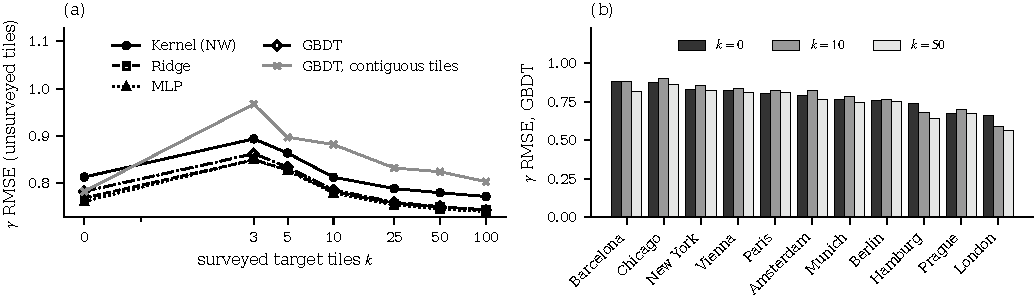
\includegraphics[width=\textwidth]{figures/fig_kshot.pdf}
\caption{(a)~Exponent RMSE against the number of surveyed target tiles.
(b)~GBDT per held-out city at $k\in\{0,10,50\}$.}
\label{fig:kshot}
\end{figure*}

\subsection{Network-level evaluation}
\label{sec:res-network}

Table~\ref{tab:network} and Fig.~\ref{fig:network} evaluate the predictors
where a planner uses them. The first row is the tile model with the true
labels (oracle), which isolates the error of the tile model itself. The
oracle has a path-loss error of \SI{\netOracle}{\decibel}, selects the
correct serving site for \assocOracle\% of the pixels (the nearest-site rule
of Proposition~\ref{prop:tilemodel}) and misjudges the SINR by
\SI{\sinrOracle}{\decibel} on average. Transferred tile parameters
reduce the path-loss error of the source median from
\SI{\netMedian}{\decibel} to \SI{\netGbdt}{\decibel} (GBDT; \dNetGbdtMedian{}
dB, better in \nNetGbdtMedian{} of \nFolds{} cities) but remain above the
oracle, and a plan of $K=5$ sites made on their map loses \regretGbdt\% of
the pixels against \regretOracle\% for the oracle.

Site-aware link transfer removes the ceiling of the tile model. Its path-loss
error is \SI{\netLink}{\decibel} (\linkMin{} to \SI{\linkMax}{\decibel}
across cities), \SI{\gainLinkGbdt}{\decibel} below tile transfer with GBDT
(95\% CI [\loNetLinkGbdt, \hiNetLinkGbdt], better in \nNetLinkGbdt{} of
\nFolds{} cities) and \SI{\gainLinkOracle}{\decibel} below the tile model
with the \emph{true} labels ([\loNetLinkOracle, \hiNetLinkOracle],
\nNetLinkOracle{} of \nFolds). It selects the correct serving site for
\assocLink\% of the pixels (\dNetLinkAssoc{} percentage points against
GBDT, in \nNetLinkAssoc{} of \nFolds{} cities), misjudges the SINR by
\SI{\sinrLink}{\decibel} on average and loses \regretLink\% of the pixels
when planning $K=5$ sites, against \regretGbdt\% for GBDT tile transfer and
\regretOracle\% for the true tile labels. The hurdle is what makes the plans
reliable: the regressor alone, which keeps every link, has the same path-loss
error but a planning regret of \regretLinkReg\%, because it lets distant,
obstructed sites cover pixels they do not reach.

\paragraph{Cell edges and dimensioning}
Table~\ref{tab:mobility} turns the maps into mobility and dimensioning
quantities. Every tile model draws the nearest-site cell pattern of
Proposition~\ref{prop:tilemodel}: its cell edges lie
\SI{\edgeGbdt}{\metre} from the true edges on average (\SI{\edgeOracle}{\metre}
with the true labels), and their total length is in error by
\edgeLenGbdt\%: the ray-traced serving pattern is fragmented by buildings and a
route crosses many more cell edges than the nearest-site pattern suggests.
Link transfer places the edges \SI{\edgeLink}{\metre} from the truth with an
edge-length error of \edgeLenLink\%. For dimensioning, the truth needs on
average \sitesNeedTrue{} of the \nSitesPerCity{} sites to cover
\covTarget\% of the pixels at \SI{140}{\decibel}. The tile models, which
cannot represent the obstruction of distant sites, predict that
\sitesNeedGbdt{} suffices (GBDT; \sitesNeedOracle{} with the true
labels, averages over the cities), and the sites they choose cover only
\sitesCovGbdt\% of the pixels in truth. Link transfer chooses
\sitesNeedLink{} on average, which cover \sitesCovLink\%; it still
under-dimensions the network, but by far less (the regressor alone:
\sitesNeedLinkReg{}, \sitesCovLinkReg\%).

The model relies on the propagation features, which account for
\linkFeatShare\% of the gain of its trees (Table~\ref{tab:importance}); the
single most important feature is the \topLinkFeat{} (\topLinkFeatShare\%),
and the three most important together account for \topThreeLinkShare\%.

\begin{table*}[!t]
\centering
\caption{Network-level evaluation on the held-out cities (mean over cities).
Oracle: tile model with the true labels. Serving site: share of pixels with the
correct serving site. Coverage: agreement of covered pixels (serving path loss
$\le\SI{130}{\decibel}$) and error of the covered share. SINR: mean absolute
error and Kolmogorov--Smirnov distance of the distributions. SE: error of mean
spectral efficiency (b/s/Hz). Regret: coverage lost by planning $K=5$ sites on
the predicted map instead of the true map. True covered share:
\covTrue\%; true mean spectral efficiency: \seTrue{}\,b/s/Hz.}
\label{tab:network}
\small\setlength{\tabcolsep}{4pt}
% generated by paper/scripts/make_assets.py
\begin{tabular}{lrrrrrrrrr}
\toprule
& \multicolumn{2}{c}{Path loss (dB)} & Serving & \multicolumn{2}{c}{Coverage 130\,dB (\%)} & \multicolumn{2}{c}{SINR} & SE & Regret \\
\cmidrule(lr){2-3}\cmidrule(lr){5-6}\cmidrule(lr){7-8}
Predictor & RMSE & bias & site (\%) & agree & $\Delta$ & MAE (dB) & KS & $\Delta$ & $K{=}5$ (\%) \\
\midrule
Tile labels (oracle) & 11.64 & +0.00 & 50.1 & 89.6 & 6.0 & 7.56 & 0.304 & \ensuremath{-}0.652 & 9.3 \\
\midrule
Source median & 14.52 & +3.68 & 50.1 & 87.9 & 8.9 & 7.18 & 0.290 & \ensuremath{-}0.668 & 32.1 \\
3GPP UMa NLoS & 22.75 & +17.29 & 50.1 & 70.2 & \ensuremath{-}16.9 & 6.92 & 0.118 & \ensuremath{-}0.213 & 8.0 \\
COST-231 Hata & 25.29 & +20.89 & 50.1 & 52.8 & \ensuremath{-}40.1 & 7.14 & 0.218 & \ensuremath{-}0.494 & 9.9 \\
Kernel (NW) & 13.02 & +1.30 & 50.1 & 88.2 & 8.4 & 7.47 & 0.296 & \ensuremath{-}0.675 & 19.0 \\
GP-ARD & 12.80 & +1.02 & 50.1 & 88.1 & 7.5 & 7.56 & 0.298 & \ensuremath{-}0.676 & 17.9 \\
$k$-NN & 12.83 & +1.12 & 50.1 & 88.4 & 8.5 & 7.56 & 0.291 & \ensuremath{-}0.665 & 28.8 \\
Ridge & 12.80 & +1.06 & 50.1 & 87.9 & 7.6 & 7.54 & 0.298 & \ensuremath{-}0.674 & 18.9 \\
CORAL + ridge & 13.08 & +2.38 & 50.1 & 87.3 & 5.5 & 7.63 & 0.316 & \ensuremath{-}0.708 & 18.3 \\
MLP & 12.76 & +1.02 & 50.1 & 88.2 & 7.8 & 7.57 & 0.297 & \ensuremath{-}0.673 & 26.5 \\
Neural encoder & 12.79 & +0.86 & 50.1 & 88.4 & 8.5 & 7.54 & 0.294 & \ensuremath{-}0.668 & 25.8 \\
GBDT & 12.80 & +0.97 & 50.1 & 88.3 & 8.2 & 7.44 & 0.294 & \ensuremath{-}0.671 & 20.6 \\
GBDT-IW & 12.82 & +0.89 & 50.1 & 88.3 & 8.1 & 7.44 & 0.293 & \ensuremath{-}0.669 & 18.7 \\
GBDT + 10 tiles & 12.75 & +0.96 & 50.1 & 88.5 & 7.7 & 7.56 & 0.299 & \ensuremath{-}0.673 & 20.4 \\
GBDT + 10 designed tiles & 12.73 & +1.25 & 50.1 & 88.3 & 7.3 & 7.52 & 0.290 & \ensuremath{-}0.643 & 19.8 \\
\midrule
Link transfer (ours) & 9.33 & \ensuremath{-}0.01 & 68.8 & 90.4 & 2.4 & 5.37 & 0.048 & \ensuremath{-}0.078 & 0.5 \\
Link, regressor only & 9.33 & \ensuremath{-}0.01 & 68.9 & 90.4 & 2.5 & 5.83 & 0.162 & \ensuremath{-}0.322 & 5.6 \\
Link + 10 tiles (ours) & 9.46 & +0.11 & 65.9 & 90.3 & 2.5 & 5.52 & 0.047 & \ensuremath{-}0.067 & 0.5 \\
Link + 10 designed tiles (ours) & 9.52 & \ensuremath{-}0.15 & 65.6 & 90.1 & 2.6 & 5.65 & 0.051 & \ensuremath{-}0.071 & 0.9 \\
\bottomrule
\end{tabular}

\end{table*}

\begin{figure*}[!t]
\centering
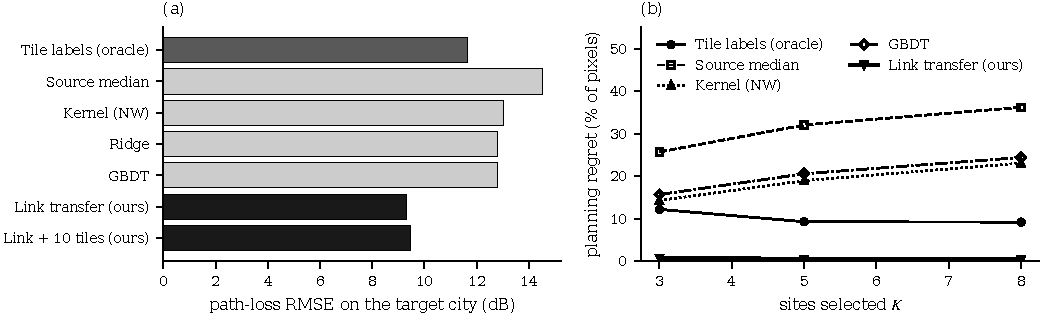
\includegraphics[width=\textwidth]{figures/fig_network.pdf}
\caption{(a)~Path-loss RMSE on the held-out cities. (b)~Planning regret against
the number of selected sites.}
\label{fig:network}
\end{figure*}

\begin{table}[!t]
\centering
\caption{Cell edges and dimensioning (mean over held-out cities). Disp.:
mean distance between true and predicted cell edges; length: relative error
of the number of cell-edge pixels. Plan: sites chosen greedily on the
predicted map until it covers \covTarget\% of the pixels at
\SI{140}{\decibel}, and the true coverage of those sites; truth: sites the
same procedure needs on the true map.}
\label{tab:mobility}
\footnotesize\setlength{\tabcolsep}{2.5pt}
% generated by paper/scripts/make_assets.py
\begin{tabular}{lrrrr}
\toprule
& \multicolumn{2}{c}{Cell edges} & \multicolumn{2}{c}{Plan for 90\%} \\
\cmidrule(lr){2-3}\cmidrule(lr){4-5}
Predictor & disp.\ (m) & length (\%) & sites & true cov.\ (\%) \\
\midrule
Tile labels (oracle) & 76 & \ensuremath{-}92 & 1.1 & 49.7 \\
\midrule
Source median & 80 & \ensuremath{-}93 & 1.0 & 56.4 \\
3GPP UMa NLoS & 80 & \ensuremath{-}93 & 5.6 & 84.0 \\
Kernel (NW) & 80 & \ensuremath{-}93 & 1.0 & 51.9 \\
GP-ARD & 80 & \ensuremath{-}93 & 1.0 & 50.7 \\
Ridge & 80 & \ensuremath{-}93 & 1.0 & 50.8 \\
GBDT & 80 & \ensuremath{-}93 & 1.0 & 47.4 \\
GBDT + 10 tiles & 80 & \ensuremath{-}93 & 1.0 & 49.3 \\
\midrule
Link transfer (ours) & 7 & \ensuremath{-}5 & 3.8 & 81.6 \\
Link, regressor only & 7 & \ensuremath{-}4 & 1.0 & 56.9 \\
Link + 10 designed tiles (ours) & 7 & \ensuremath{-}3 & 3.9 & 81.9 \\
\midrule
Truth & 0 & 0 & 6.7 & 90+ \\
\bottomrule
\end{tabular}

\end{table}

\begin{table}[!t]
\centering
\caption{Link transfer: the ten features with the largest share of the total
split gain (mean over folds and seeds).}
\label{tab:importance}
\small
% generated by paper/scripts/make_assets.py
\begin{tabular}{lr}
\toprule
Feature & gain share (\%) \\
\midrule
knife-edge loss & 22.9 \\
max.\ excess height & 19.7 \\
buildings crossed & 17.4 \\
log distance & 11.7 \\
blocked fraction & 8.5 \\
length over buildings & 5.9 \\
horizontal distance & 2.4 \\
built fraction, 50\,m & 1.8 \\
receiver building height & 1.8 \\
site height & 1.6 \\
\bottomrule
\end{tabular}

\end{table}

\subsection{Survey design for site calibration}
\label{sec:res-survey}

Calibrating the per-site offsets of the link model from surveyed tiles does
not improve it (Table~\ref{tab:survey}). With ten random tiles the path-loss
error rises from \SI{\svPlZero}{\decibel} to \SI{\svPlRTen}{\decibel}
(\dNetLinkTen{} dB, worse in every city), and with fifty designed tiles it is
\SI{\svPlDFifty}{\decibel}; the design of Proposition~\ref{prop:survey},
which maximises the variance reduction of the offsets, is not better than
random tiles. This indicates that the zero-shot link model has little
systematic per-site error left for a survey of this size to remove, while an
offset estimated from the links of a few tiles transmits their local
residuals to the whole cell. A survey is better
spent on the target quantity itself, as the next section does.

\begin{table}[!t]
\centering
\caption{Per-site calibration of the link model from $k$ surveyed tiles:
random tiles (mean of ten draws) and the survey design of
Proposition~\ref{prop:survey}. PL: path-loss RMSE; serv.: serving-site
accuracy; regret: $K=5$. Means over the held-out cities. Zero-shot link
model: \SI{\svPlZero}{\decibel}, \svAssocZero\%, \svRegZero\%.}
\label{tab:survey}
\footnotesize\setlength{\tabcolsep}{2.5pt}
% generated by paper/scripts/make_assets.py
\begin{tabular}{rrrrrrr}
\toprule
& \multicolumn{3}{c}{Random survey} & \multicolumn{3}{c}{Designed survey} \\
\cmidrule(lr){2-4}\cmidrule(lr){5-7}
$k$ & PL (dB) & serv.\ (\%) & regret (\%) & PL (dB) & serv.\ (\%) & regret (\%) \\
\midrule
10 & 9.46 & 65.9 & 0.5 & 9.52 & 65.6 & 0.9 \\
25 & 9.35 & 67.6 & 0.5 & 9.46 & 66.0 & 0.7 \\
50 & 9.30 & 69.1 & 0.5 & 9.44 & 67.0 & 0.5 \\
\bottomrule
\end{tabular}

\end{table}

\subsection{Certified coverage}
\label{sec:res-certified}

Table~\ref{tab:certified} applies Proposition~\ref{prop:certify}. For every
predictor the bound $\hat q_t$ holds in \certValidLink{} of \nFolds{} cities, as the guarantee of at least \certLevel{} requires. At
$\alpha=0.1$ and \SI{140}{\decibel}, the certificate of link transfer needs a
margin of only \SI{\certQLink}{\decibel} and certifies \certClaimLink\% of
the pixels, with \certFalseLink\% falsely claimed; the true covered share is
\certTrueCov\%. Tile transfer needs larger margins and certifies less: GBDT
\certClaimGbdt\% (margin \SI{\certQGbdt}{\decibel}), the source median
\certClaimMedian\% and even the true tile labels \certClaimOracle\%. The
naive claim without a margin covers almost every pixel but is wrong for
\certNaiveFalseLink\% (link) to \certNaiveFalseGbdt\% (GBDT) of them, with no
stated risk. The accuracy of a transfer model thus translates directly
into the coverage an operator can promise at a stated risk.

\begin{table*}[!t]
\centering
\caption{Certified coverage (Proposition~\ref{prop:certify}), mean over
held-out cities. $\hat q_t$: margin from the other cities; valid: cities in
which $q_t\le\hat q_t$ (of \nFolds); $r_p\le\hat q_t$: share of pixels within
the margin; certified claim: share claimed covered and share claimed but not
covered; naive claim: without a margin; covered: true covered share.}
\label{tab:certified}
\small\setlength{\tabcolsep}{4pt}
% generated by paper/scripts/make_assets.py
\begin{tabular}{lrrrrrrrr}
\toprule
& & & & \multicolumn{2}{c}{Certified claim} & \multicolumn{2}{c}{Naive claim} & \\
\cmidrule(lr){5-6}\cmidrule(lr){7-8}
Predictor & $\hat q_t$ (dB) & valid & $r_p\le\hat q_t$ (\%) & claimed (\%) & false (\%) & claimed (\%) & false (\%) & covered (\%) \\
\midrule
\multicolumn{9}{l}{\emph{$\alpha=0.1$, $L=\SI{140}{\decibel}$, bound holding with probability $\ge 10/11$}} \\
Tile labels (oracle) & 13.4 & 10 & 93.9 & 88.2 & 1.79 & 99.9 & 3.62 & 96.3 \\
Source median & 22.2 & 10 & 95.5 & 60.5 & 1.60 & 100.0 & 3.68 & 96.3 \\
3GPP UMa NLoS & 14.6 & 10 & 95.3 & 55.6 & 1.32 & 95.5 & 3.48 & 96.3 \\
Kernel (NW) & 19.3 & 10 & 95.7 & 72.3 & 1.44 & 100.0 & 3.68 & 96.3 \\
Ridge & 17.8 & 10 & 95.1 & 77.6 & 1.60 & 100.0 & 3.68 & 96.3 \\
GBDT & 17.6 & 10 & 95.1 & 78.3 & 1.66 & 100.0 & 3.68 & 96.3 \\
Link transfer (ours) & 9.8 & 10 & 93.9 & 92.0 & 1.79 & 98.3 & 3.11 & 96.3 \\
Link, regressor only & 10.3 & 10 & 94.0 & 91.3 & 1.69 & 100.0 & 3.68 & 96.3 \\
\multicolumn{9}{l}{\emph{$\alpha=0.1$, $L=\SI{140}{\decibel}$, bound holding with probability $\ge 9/11$}} \\
Tile labels (oracle) & 13.2 & 9 & 93.7 & 88.9 & 1.88 & 99.9 & 3.62 & 96.3 \\
Source median & 22.1 & 9 & 95.4 & 61.0 & 1.64 & 100.0 & 3.68 & 96.3 \\
3GPP UMa NLoS & 14.3 & 9 & 95.1 & 56.5 & 1.36 & 95.5 & 3.48 & 96.3 \\
Kernel (NW) & 18.1 & 9 & 94.8 & 77.2 & 1.80 & 100.0 & 3.68 & 96.3 \\
Ridge & 15.2 & 9 & 93.4 & 86.7 & 2.26 & 100.0 & 3.68 & 96.3 \\
GBDT & 16.3 & 9 & 94.2 & 83.2 & 2.00 & 100.0 & 3.68 & 96.3 \\
Link transfer (ours) & 8.9 & 9 & 93.1 & 93.5 & 2.03 & 98.3 & 3.11 & 96.3 \\
Link, regressor only & 9.8 & 9 & 93.4 & 92.4 & 1.88 & 100.0 & 3.68 & 96.3 \\
\multicolumn{9}{l}{\emph{$\alpha=0.05$, $L=\SI{140}{\decibel}$, bound holding with probability $\ge 10/11$}} \\
Tile labels (oracle) & 18.7 & 10 & 97.3 & 71.0 & 0.75 & 99.9 & 3.62 & 96.3 \\
Source median & 27.5 & 10 & 98.0 & 32.4 & 0.64 & 100.0 & 3.68 & 96.3 \\
3GPP UMa NLoS & 20.4 & 10 & 97.9 & 34.2 & 0.63 & 95.5 & 3.48 & 96.3 \\
Kernel (NW) & 24.5 & 10 & 98.1 & 48.8 & 0.50 & 100.0 & 3.68 & 96.3 \\
Ridge & 22.5 & 10 & 97.7 & 57.8 & 0.64 & 100.0 & 3.68 & 96.3 \\
GBDT & 22.3 & 10 & 97.6 & 58.8 & 0.68 & 100.0 & 3.68 & 96.3 \\
Link transfer (ours) & 14.5 & 10 & 97.1 & 82.7 & 0.82 & 98.3 & 3.11 & 96.3 \\
Link, regressor only & 14.7 & 10 & 97.1 & 82.3 & 0.78 & 100.0 & 3.68 & 96.3 \\
\bottomrule
\end{tabular}

\end{table*}

\subsection{Robustness}
\label{sec:res-robust}

\paragraph{Tile size}
Table~\ref{tab:tilesize} repeats the tile pipeline for
$G_s\in\{50,100,200\}$\,m; $G_s=\SI{100}{\metre}$ reproduces the main
results exactly. Larger tiles give more precise labels (cluster-robust
standard error \tsSeFifty, \tsSeHundred{} and \tsSeTwoHundred) and a smaller
exponent error (GBDT \tsGammaFifty, \tsGammaHundred{} and \tsGammaTwoHundred),
but a coarser map: the path-loss error of the oracle grows from
\SI{\tsOracleFifty}{\decibel} to \SI{\tsOracleTwoHundred}{\decibel}, and that
of GBDT tile transfer stays between \SI{\tsGbdtFifty}{\decibel} and
\SI{\tsGbdtTwoHundred}{\decibel}. The serving-site accuracy of the tile model
is \tsAssocMin--\tsAssocMax\% at every size, as
Proposition~\ref{prop:tilemodel} implies. No tile size approaches link
transfer.

\paragraph{Path-loss cut-off}
Between \censMin\% and \censMax\% of the (pixel, site) pairs of the labelled
tiles lie beyond the cut-off (Table~\ref{tab:censoring}). The labels depend
on this dynamic range: lowering the cut-off to \SI{140}{\decibel} changes the
median tile exponent by \censDgOneForty{} and to \SI{130}{\decibel} by
\censDgOneThirty, and a Tobit fit that also uses the censored pairs gives
slopes larger than the least-squares slopes by a median of \censTobitMin{} to
\censTobitMax{} across the cities (\censTobitTiles{} tiles). The tile exponent thus
depends on the dynamic range of the measurements, not only on the
environment, which is a further reason to model links, and to model the cut-off
explicitly as the hurdle of the link model does.

\paragraph{Network size}
On the network of the first \nSitesSmall{} sites (Table~\ref{tab:density}),
the ranking is unchanged: the oracle has a path-loss error of
\SI{\smallNetOracle}{\decibel}, GBDT tile transfer \SI{\smallNetGbdt}{\decibel}
and link transfer \SI{\smallNetLink}{\decibel}, with serving-site accuracies
of \smallAssocOracle\%, \smallAssocGbdt\% and \smallAssocLink\%.

\begin{table*}[!t]
\centering
\caption{Tile size. Tiles per city, median shrinkage weight and standard error
of the exponent (iid and cluster-robust, RMS over tiles); zero-shot exponent
RMSE of the source median and GBDT; network path-loss RMSE of the tile labels
(oracle) and of GBDT tile transfer; serving-site accuracy of the tile model.
Means over the held-out cities.}
\label{tab:tilesize}
\small
% generated by paper/scripts/make_assets.py
\begin{tabular}{rrrrrrrrrr}
\toprule
& & & \multicolumn{2}{c}{$\mathrm{se}(\gamma)$} & \multicolumn{2}{c}{$\gamma$ RMSE} & \multicolumn{2}{c}{PL RMSE (dB)} & \\
\cmidrule(lr){4-5}\cmidrule(lr){6-7}\cmidrule(lr){8-9}
$G_s$ (m) & tiles/city & med.\ $w_t$ & iid & cluster & median & GBDT & oracle & GBDT & serv.\ (\%) \\
\midrule
50 & 3470 & 0.38 & 0.234 & 0.540 & 0.985 & 0.888 & 11.19 & 12.67 & 50.1 \\
100 & 948 & 0.37 & 0.141 & 0.456 & 0.871 & 0.782 & 11.64 & 12.80 & 50.1 \\
200 & 244 & 0.38 & 0.088 & 0.369 & 0.716 & 0.619 & 12.09 & 13.05 & 50.1 \\
\bottomrule
\end{tabular}

\end{table*}

\begin{table*}[!t]
\centering
\caption{Path-loss cut-off. Share of (pixel, site) pairs of the labelled
tiles beyond the \SI{\maxPl}{\decibel} cut-off and of links above
\SI{140}{\decibel}; median change of the tile exponent when the cut-off is
lowered to 140 and \SI{130}{\decibel}; for random tiles, median and 90th
percentile of the Tobit minus the least-squares slope.}
\label{tab:censoring}
\small
% generated by paper/scripts/make_assets.py
\begin{tabular}{lrrrrrrr}
\toprule
& censored & \multicolumn{3}{c}{Lower cut-off} & \multicolumn{3}{c}{Tobit vs least squares} \\
\cmidrule(lr){3-5}\cmidrule(lr){6-8}
City & pairs (\%) & links $>$140 (\%) & $\Delta\gamma_{140}$ & $\Delta\gamma_{130}$ & tiles & med.\ $\Delta\gamma$ & q90 \\
\midrule
Amsterdam & 56.8 & 18.4 & \ensuremath{-}0.572 & \ensuremath{-}1.141 & 300 & +3.746 & +6.802 \\
Barcelona & 61.0 & 18.7 & \ensuremath{-}0.486 & \ensuremath{-}0.893 & 300 & +4.284 & +7.509 \\
Berlin & 43.5 & 17.3 & \ensuremath{-}0.646 & \ensuremath{-}1.261 & 300 & +3.256 & +6.938 \\
Chicago & 40.5 & 17.9 & \ensuremath{-}0.640 & \ensuremath{-}1.226 & 300 & +3.536 & +6.698 \\
Hamburg & 35.5 & 15.0 & \ensuremath{-}0.504 & \ensuremath{-}1.066 & 300 & +2.113 & +3.886 \\
London & 46.9 & 14.6 & \ensuremath{-}0.470 & \ensuremath{-}0.855 & 300 & +2.946 & +5.014 \\
Munich & 54.7 & 20.1 & \ensuremath{-}0.583 & \ensuremath{-}1.184 & 300 & +3.157 & +5.333 \\
New York & 53.8 & 23.8 & \ensuremath{-}0.621 & \ensuremath{-}1.119 & 300 & +4.492 & +7.343 \\
Paris & 63.1 & 18.3 & \ensuremath{-}0.598 & \ensuremath{-}1.006 & 300 & +4.266 & +8.338 \\
Prague & 55.8 & 21.5 & \ensuremath{-}0.729 & \ensuremath{-}1.366 & 300 & +3.500 & +5.315 \\
Vienna & 66.4 & 22.9 & \ensuremath{-}0.527 & \ensuremath{-}0.980 & 300 & +4.146 & +7.915 \\
\bottomrule
\end{tabular}

\end{table*}

\begin{table*}[!t]
\centering
\caption{Network size: the same predictors on the \nSitesPerCity-site and on
the \nSitesSmall-site network (mean over held-out cities). PL: path-loss
RMSE; serv.: serving-site accuracy; SINR: mean absolute error; regret: $K=5$.}
\label{tab:density}
\small
% generated by paper/scripts/make_assets.py
\begin{tabular}{lrrrrrrrr}
\toprule
& \multicolumn{4}{c}{20 sites} & \multicolumn{4}{c}{10 sites} \\
\cmidrule(lr){2-5}\cmidrule(lr){6-9}
Predictor & PL (dB) & serv.\ (\%) & SINR (dB) & regret (\%) & PL (dB) & serv.\ (\%) & SINR (dB) & regret (\%) \\
\midrule
Tile labels (oracle) & 11.64 & 50.1 & 7.56 & 9.3 & 11.67 & 51.3 & 8.05 & 6.3 \\
\midrule
Source median & 14.52 & 50.1 & 7.18 & 32.1 & 14.91 & 51.3 & 7.85 & 27.0 \\
3GPP UMa NLoS & 22.75 & 50.1 & 6.92 & 8.0 & 23.87 & 51.3 & 8.04 & 4.5 \\
Kernel (NW) & 13.02 & 50.1 & 7.47 & 19.0 & 13.20 & 51.3 & 8.07 & 18.7 \\
GP-ARD & 12.80 & 50.1 & 7.56 & 17.9 & 12.95 & 51.3 & 8.12 & 12.7 \\
Ridge & 12.80 & 50.1 & 7.54 & 18.9 & 12.96 & 51.3 & 8.11 & 14.7 \\
GBDT & 12.80 & 50.1 & 7.44 & 20.6 & 12.95 & 51.3 & 8.04 & 16.1 \\
Link transfer (ours) & 9.33 & 68.8 & 5.37 & 0.5 & 9.22 & 68.3 & 6.22 & 0.4 \\
\bottomrule
\end{tabular}

\end{table*}

\subsection{Statistical summary}
\label{sec:res-stats}

Tables~\ref{tab:stats-param} and~\ref{tab:stats-net} (\ref{app:stats}) list
all \nStatsRows{} city-level comparisons. Link transfer improves on GBDT tile
transfer in path loss, serving site, coverage agreement and planning regret
in all \nFolds{} cities, and on the tile model with the true labels in path
loss, serving site and planning regret in all \nFolds{} cities; these
comparisons remain significant after Holm's correction. At the parameter
level the evidence is weaker: of the \nZeroShotTotal{} comparisons of a
transfer operator with the source median, no improvement survives Holm's
correction at eleven cities, whereas the gain of GP-ARD over kernel transfer
does.
